\documentclass[tikz,border=10pt,dvipsnames]{standalone}
\usetikzlibrary{
  arrows.meta,                        % for arrow tips
  backgrounds,                        % for background layer
  bending,
  ext.paths.ortho,                    % for ortho paths
  positioning,
  ext.positioning-plus,               % for 
  ext.node-families.shapes.geometric, % loads ext.node-families and
% shapes.geometric,                   % for ellipse
  calc,                               % for ($$)
  backgrounds %https://tex.stackexchange.com/questions/230224/how-to-change-the-background-color-in-tikz
}
% node styles
\tikzstyle{flowstep} = [rectangle, draw, text centered, rounded corners, minimum height=2em]
\tikzstyle{semistep}=[flowstep,fill=green!20]
\tikzstyle{fullstep}=[flowstep,fill=blue!20]
\tikzstyle{concept}=[flowstep,fill=orange!20]
\tikzstyle{simstep}=[flowstep,fill=yellow!20]
\tikzstyle{veristep}=[flowstep,fill=BurntOrange!60]
\tikzstyle{designstep}=[flowstep,fill=pink!50]
\tikzstyle{expensivestep}=[flowstep,fill=red!30]
% edge styles
\tikzstyle{happypath}=[->,rounded corners,thick,ForestGreen!75!white]
% no arrow
\tikzstyle{unhappypathna}=[rounded corners,thick,BrickRed!75!white]
\tikzstyle{unhappypath}=[->,unhappypathna]
\tikzstyle{veryunhappypath}=[rounded corners,thick,Red,->]
\tikzset{
  fill fraction/.style n args={3}{path picture={
 \fill[#1] (path picture bounding box.south west) rectangle
 ($(path picture bounding box.north west)!#3!(path picture bounding box.north
 east)$);
 \fill[#2] (path picture bounding box.south east) rectangle
 ($(path picture bounding box.north west)!#3!(path picture bounding box.north
 east)$);}}
}

\begin{document}
%source: andreas burg https://ee222-winter19-01.courses.soe.ucsc.edu/system/files/attachments/EE222W19_Lect1_Part2-Introduction.pdf

% TODO add an image to each level, unveil in 2nd step all at once
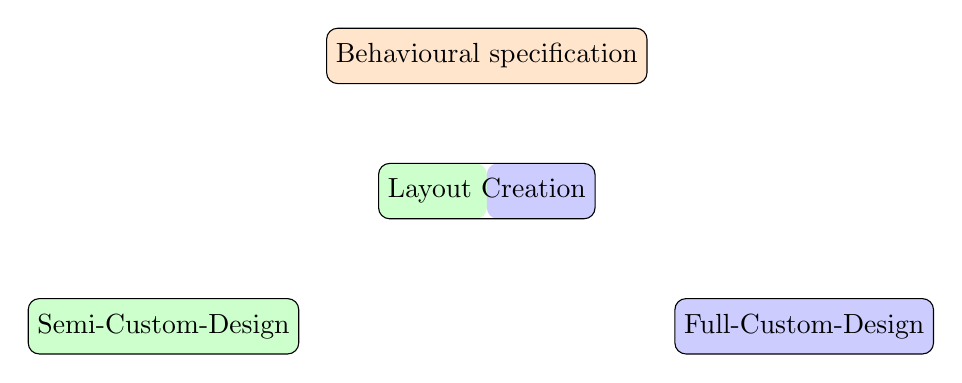
\begin{tikzpicture}
  % first flow nodes
\node[concept](conceptidea) at (3,0) {Behavioural specification};
\node[flowstep,fill fraction={green!20}{blue!20}{0.5}](layout)[below=of conceptidea]{Layout Creation}; % can either be full custom or semi custom, will involve netlist,floor plan place and route
\node[semistep](semicustom) [below left=of layout,fill=green!20] {Semi-Custom-Design};
\node[fullstep](fullcustom) [below right=of layout,fill=blue!20] {Full-Custom-Design};

%% in semicustom: synthesizeable behavioural sim, synthesis (opt + map), place + route
% in full custom: decide on topology,size, manual place + route
% => same steps, just 
% *very* unhappy paths manual/finegrained vs automated
% we already have good P+R and they are getting better
% how do we think about topologies as a unit instead of hierarchical macros?
\end{tikzpicture}
\end{document}
